\mysection{Introduzione}

\myframe{Documento}{frame:doc1099}{
\begin{center}
\begin{tabular}{cc}
  \multicolumn{2}{c}{\only<2>{1601}}\\
  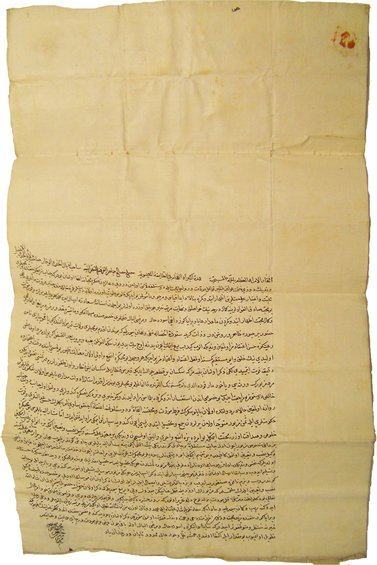
\includegraphics{rdoc1099r-rid.jpg} &
  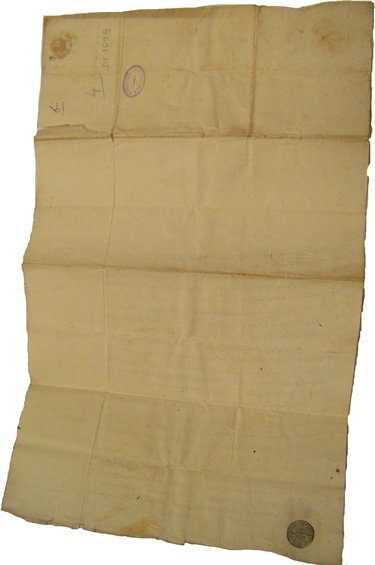
\includegraphics{rdoc1099v-rid.jpg} \\
\end{tabular}
\end{center}
}

\myframe{Regesto}{frame:regesto}{
  \begin{center}
    {\scriptsize
      
      \begin{tabular}{p{2cm}cr}
        &Cose turchi&N$^\text{o}$ 379\\[2mm]
        &Sine data&\\[2mm]
        \multicolumn{3}{c}{
          \parbox{7.5cm}{Lettera in  turco diretta al  
            {\only<3>{\color{evidenzia}\bf}Doge di Venezia}
            da {\only<2>{\color{evidenzia}\bf}Gefer Bassà fu Beglierbei di Cipro} nella quale si lagna
            della    perdita     fatta    di    alcune     balle    di
            Bombace.}}\\
        &Originale e traduzione.&\\
      \end{tabular}
    }

    \parbox[b][6cm][c]{10cm}{\centering
      \only<1>{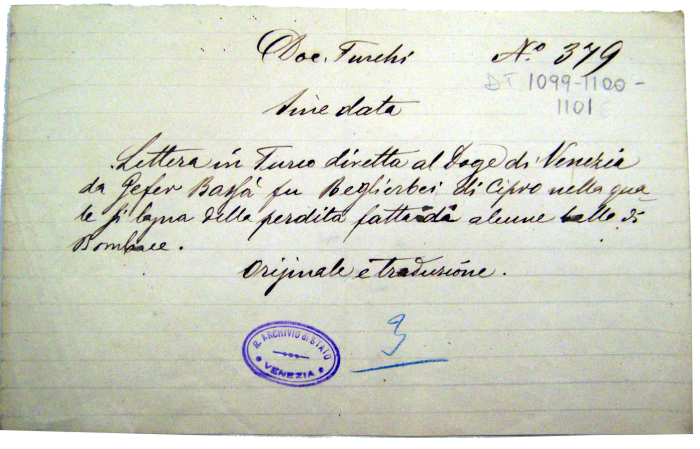
\includegraphics[scale=0.28]{regesto.png}}
      \only<2>{\begin{tabular}[b]{cc}
          \includegraphics[scale=0.18]{documenti/vecellio295.png}&
          \includegraphics[scale=0.3]{ritratti/nadiri-rid.jpg}\\ 
          \resizebox{3cm}{!}{\parbox{8cm}{{\sc Cesare Vecellio}, {\it Habiti antichi et moderni di tutto il mondo}, Venezia, 1598}}
          & \resizebox{3cm}{!}{\parbox{8cm}{{\it  Musicisti di fronte  a Mehmed  III}, Topkapı  Sarayı Müzesi,
              inv.  H889, f.  8, XVII  sec.}} \\
        \end{tabular}}
      \only<3>{\begin{tabular}[b]{lr}
          \includegraphics[scale=0.25]{ritratti/marino_grimani.jpg}&
          \begin{tabular}[b]{r}
            {\tiny Marino Grimani}\\
            {\tiny 1532-1605, doge dal 1595}\\[0.5cm]
            \resizebox{3cm}{!}{\parbox{8cm}{Gabriele Caliari, {\it Il doge Marino Grimani riceve l'ambasciatore persiano}, Venezia, Palazzo Ducale, XVI sec.}}\\
          \end{tabular}\\
        \end{tabular}
      }
    }
    
  \end{center}
}

\myframe{Lingua}{frame:lingua}{
  \begin{tikzpicture}[x=2cm,y=2cm,node distance=1,
      linea/.style={line width=2pt,draw=red},
      lineb/.style={line width=2pt,draw=black},
      linec/.style={line width=2pt,draw=white},
    ]
    \node (docpos) {\includegraphics{img/doc-rid.jpg}};
    \node (poesiapos) at ($(docpos)+(3,1)$) {};
    \node (bazarpos) at ($(docpos)+(3,-1)$) {};
    \only<2->{
      \node (a) at (poesiapos) {\includegraphics[scale=0.5]{img/poesia-rid.jpg}};
    }
    \only<2>{
      \draw[<->,linea] (a) to (docpos);
    }
    \only<3->{
      \node (b) at (bazarpos) {\includegraphics[scale=0.5]{img/bazar-rid.jpg}};
    }
    \only<3> {
      \draw[<->,linea] (b) to (docpos);
      \draw[<->,lineb] (a) to (docpos);
    }
    \only<4>{
      \draw[linea] ($(docpos)+(-1,-1.5)$) rectangle ($(docpos)+(1,1.5)$);
      \draw[->,linea] ($(docpos)+(1,0)$) to ($(docpos)+(3,0)$);
    }
  \end{tikzpicture}
}

